%%%%%%%%%%%%%%%%%%%%%%%%%%%%%%%%%%%%%%%%%%%%%%%%%%%%%%%%%%%%%%%%%%%%%%%%%%%%%%%%
%2345678901234567890123456789012345678901234567890123456789012345678901234567890
%        1         2         3         4         5         6         7         8
%
\documentclass[letterpaper, 10 pt, conference]{ieeeconf}  % Comment this line out if you need a4paper

%\documentclass[a4paper, 10pt, conference]{ieeeconf}      % Use this line for a4 paper

\IEEEoverridecommandlockouts                              % This command is only needed if 
                                                          % you want to use the \thanks command

\overrideIEEEmargins                                      % Needed to meet printer requirements.

% See the \addtolength command later in the file to balance the column lengths
% on the last page of the document

% The following packages can be found on http:\\www.ctan.org
\usepackage{graphics} % for pdf, bitmapped graphics files
\usepackage{graphicx} % for pdf, bitmapped graphics files
\usepackage{epsfig} % for postscript graphics files
%\usepackage{mathptmx} % assumes new font selection scheme installed
%\usepackage{times} % assumes new font selection scheme installed
%\usepackage{amsmath} % assumes amsmath package installed
%\usepackage{amssymb}  % assumes amsmath package installed
\usepackage{subfig}
\usepackage{color}
\usepackage{url}
\usepackage{caption}

% Suggested by Michele:
%\documentclass[letterpaper, 10 pt, conference]{ieeeconf}  % Comment this line out
%\usepackage{amssymb}
%\usepackage{amsmath}
%\usepackage{graphics}
%\usepackage{blkarray}
%\usepackage{booktabs}
%\usepackage{xcolor} 
%\usepackage{caption}
%\usepackage{multirow}
%\usepackage{comment}
%\usepackage{epstopdf}
%\usepackage{epsfig} % for postscript graphics files
%\usepackage{tikz}
%\usepackage{todonotes}
%\usetikzlibrary{arrows,matrix,positioning}
%\graphicspath{{./figures/}}
%\usepackage{caption}
%\usepackage{soul}
%\usepackage{url}

%mods
\DeclareCaptionLabelSeparator{periodspace}{.\quad}
\captionsetup{font=small,labelsep=periodspace,singlelinecheck=true}
\captionsetup[sub]{font=small,singlelinecheck=true}
\renewcommand\thesubfigure{(\alph{subfigure})}

%\usepackage{cite}
                             % if you need a4paper
%\documentclass[a4paper, 10pt, conference]{ieeeconf}      % Use this line for a4
                                                          % paper
\IEEEoverridecommandlockouts                              % This command is only
                                                          % needed if you want to
                                                          % use the \thanks command
\overrideIEEEmargins
% See the \addtolength command later in the file to balance the column lengths
% on the last page of the document

\graphicspath{{images/}}

\title{\LARGE \bf
KTH-3D-TOTAL: A 3D Dataset for Discovering Spatial Structures for Long-Term Autonomous
 Learning
}

\author{Akshaya Thippur$^{1}$, Rares Ambrus$^{1}$, Gaurav Agrawal$^{2}$, Adri\`a Gallart del Burgo$^{1}$, Janardhan Haryadi Ramesh$^{2}$, \\Mayank Kumar Jha$^{2}$, Malepati Bala Siva Sai Akhil$^{2}$,  Nishan Bhavanishankar Shetty$^{2}$, \\John Folkesson $^{1}$ and Patric Jensfelt$^{1}$% <-this % stops a space
\thanks{$^{1}$ KTH Royal Institute of Technology, Stockholm:
        {\tt\small akshaya@kth.se}}%
\thanks{$^{2}$ M.S. Ramaiah Institute of Technology, V.T.U, Bangalore}%
}

\begin{document}

\maketitle
\thispagestyle{empty}
\pagestyle{empty}

%%%%%%%%%%%%%%%%%%%%%%%%%%%%%%%%%%%%%%%%%%%%%%%%%%%%%%%%%%%%%%%%%%%%%%%%%%%%%%%%
\begin{abstract}

Long-term autonomous learning of human environments entails modelling 
and generalizing over distinct variations in: object instances in different scenes, 
and different scenes with respect to space and time. It is crucial for the 
robot to recognize the structure and context in spatial arrangements and 
exploit these to learn models which capture the essence of these distinct variations.
Table-tops posses a typical structure repeatedly seen in human environments
and are identified by characteristics of being personal spaces of diverse
functionalities and dynamically changing due to human interactions. In this
paper, we present a 3D dataset of 20 office table-tops observed 3 times a 
day for 19 days (1140 scenes), manually annotated with 18 different object 
classes, including multiple instances. We analyse the dataset to discover 
spatial structures and patterns in their variations. The dataset can, for example, be used 
to study the spatial relations between objects and long-term environment models 
for applications such as activity recognition, context and functionality estimation and anomaly detection.

\end{abstract}

%%%%%%%%%%%%%%%%%%%%%%%%%%%%%%%%%%%%%%%%%%%%%%%%%%%%%%%%%%%%%%%%%%%%%%%%%%%%%%%%

\section{Introduction}
\label{sec:Introduction}

A complete understanding of a scene includes information on not only 
what objects are in the scene but also on their relative arrangement in
the scene. For a robot to recognize a context it should take this into
account.  Our research work involves developing
a mobile service robot for long-term autonomy in indoor human
environments, from offices to hospitals.  The ability for a robot to
run for weeks or months in its task environment opens up a new range
of possibilities in terms of learning capabilities. In particular, the
robot would expected to learn to perform an assigned task that is
repetitive with weaning supervision and human interaction. The
contextual knowledge the robot can gain from the repeated attempts can
make it learn so that it's subsequent attempts on the same task are
improved in accuracy and efficiency.

In this paper we study spatial understanding derived from the 
configuration of objects in a scene. Whilst objects often change 
in position, their overall arrangement typically have some regularity 
over time as influenced by the context and functionality of that 
part of space. For example, there is a general structure in office 
employee table-tops to that of cafeteria table-tops or kitchen table-tops.
The differences derive from the variety of objects and their 
group-configurations on the table-tops with respect to time -- hours, 
days, weeks, months etc. For example: Office tables typically 
have monitors, keyboards, mouse along with papers and pens 
and coffee mugs arranged such that the monitors can be viewed, the 
keyboard typed at and the mouse easily accessed from the keyboard. 
The spatial configurations vary in particular instances and the 
arrangement change gradually over many days and minutely at different 
times of the day; However, cafeteria tables have cutlery, jugs, food, 
napkins etc.\ configurations of which don't vary over many days, 
weeks or years but vary in content and presence according to different 
times of every day. It is this structure and it's variants that we aim 
to exploit in order to improve the understanding of space.

Such structures have been exploited before in the literature for a
number of different applications, such as object recognition, activity
recognition, image retrieval and objects search. The intuition is that:
bluntly modelling the absolute positions of objects, is likely to fail
because such a model is improbable to generalise across a range of
different scenes from numerous observations w.r.t.\ time and instance. Instead
qualitative \emph{relational} models of space, i.e. ways of encoding
the qualitative position of a target object relative to the position
of one or more landmark objects are investigated. For example, "the
chair is \textit{at} the table" and "the pillow \textit{on} the bed". 
The exact coordinates of these objects are semantically irrelevant. We believe that 
representations that are to support long-term autonomy and ability 
to generalize knowledge require such rough discretizations of metric 
measurement space forming a "feature set" inherently encapsulating the generality
of structure.

The main contribution of this paper is the quantitative and qualitative analysis of
indoor environments to characterise some of these structures. This is
an important contribution if one wants to design a representation to
build a model of space and to reason about space.  The prevailing
approach has been to assume structures exist and define a set of
descriptors/features that capture different aspects of these. We
instead propose to carefully study the structures and do so over long
periods of time and across several similar scenes to be able to characterise the
dynamics and variability. The output of this paper can thus serve as
the foundation for designing efficient representations and inference
algorithms. To limit the scope, we study table-top scenes in this
paper. As a basis for our study, we have constructed a large, manually annotated 
benchmark 3D dataset of office type table-top scenes called \textit{\textbf{KTH-3D-T}able-T\textbf{o}ps Dataset for Long \textbf{T}erm
  \textbf{A}utonomous \textbf{L}earning} (KTH-3D-TOTAL)\footnote{\url{http://www.cas.kth.se/data/KTH-3D-TOTAL/}} observing
the same set of select tables, over many times a day and over many
days in a month. Objects-of-interest have been manually annotated in
3D to provide ground truth data.

The rest of the paper is composed in the following way: We survey the related work in Section~\ref{sec:Related Work}. In Section~\ref{sec:Dataset} we exhibit KTH-3D-TOTAL in depth and provide an 
analysis of it in Section~\ref{sec:Analysis}. We summarize and conclude in Section~\ref{sec:Conclusions}.


%%%%%%%%%%%%%%%%%%%%%%%%%%%%%%%%%%%%%%%%%%%%%%%%%%%%%%%%%%%%%%%%%%%%%%%%%%%%%%%%

\begin{figure*}[bhtp]
\begin{center}
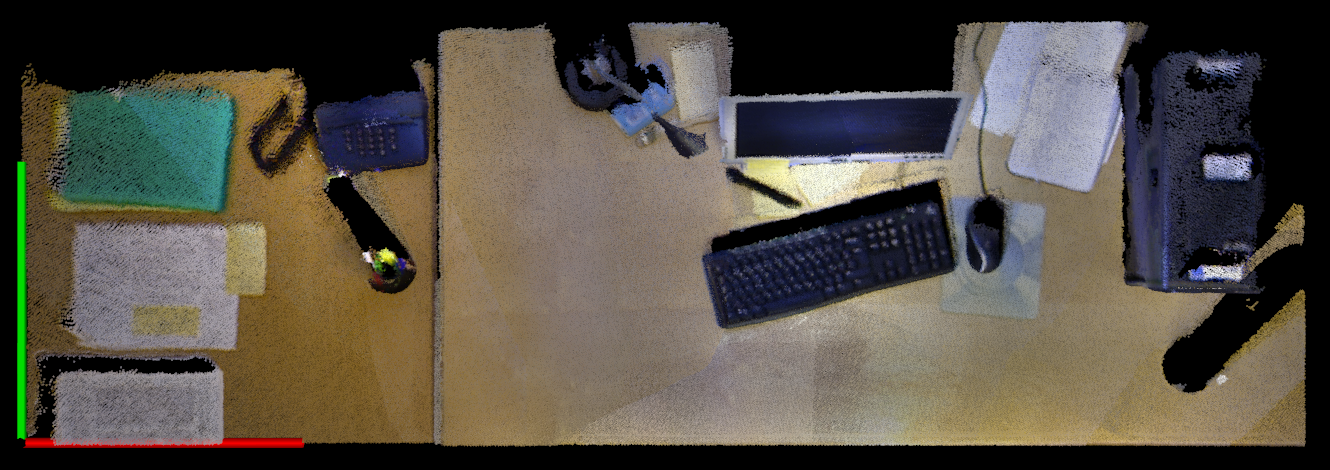
\includegraphics[height=2.5cm]{David_Mor_131110} \quad
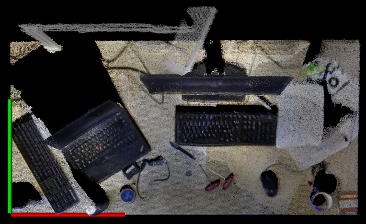
\includegraphics[height=2.5cm]{Nils_Mor_131111} \quad
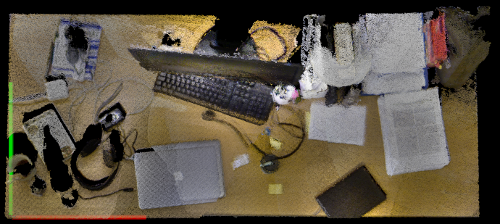
\includegraphics[height=2.5cm]{Puren_Eve_131029}\\ \smallskip
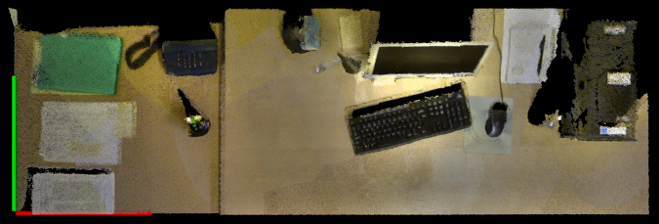
\includegraphics[height=2.5cm]{David_Eve_131110} \enskip
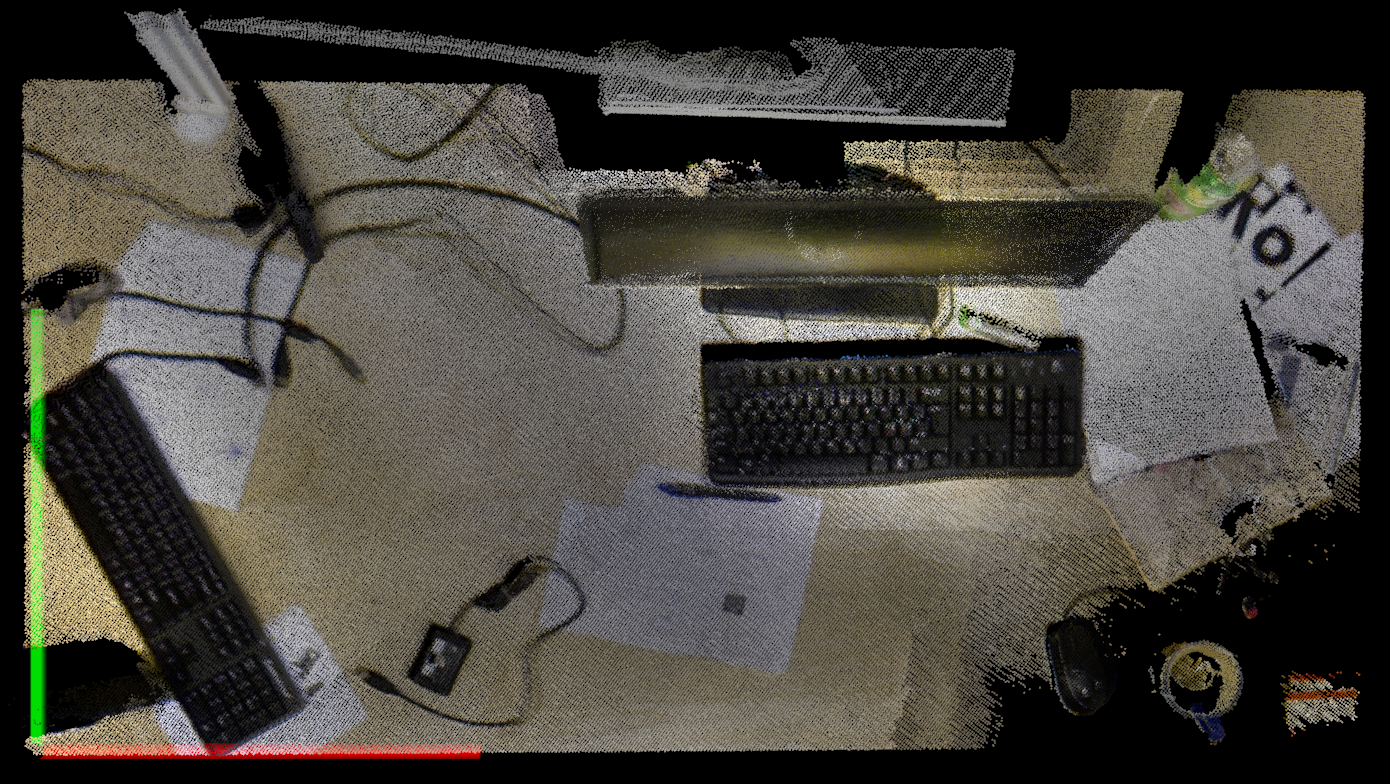
\includegraphics[height=2.5cm]{Nils_Eve_131111} \enskip
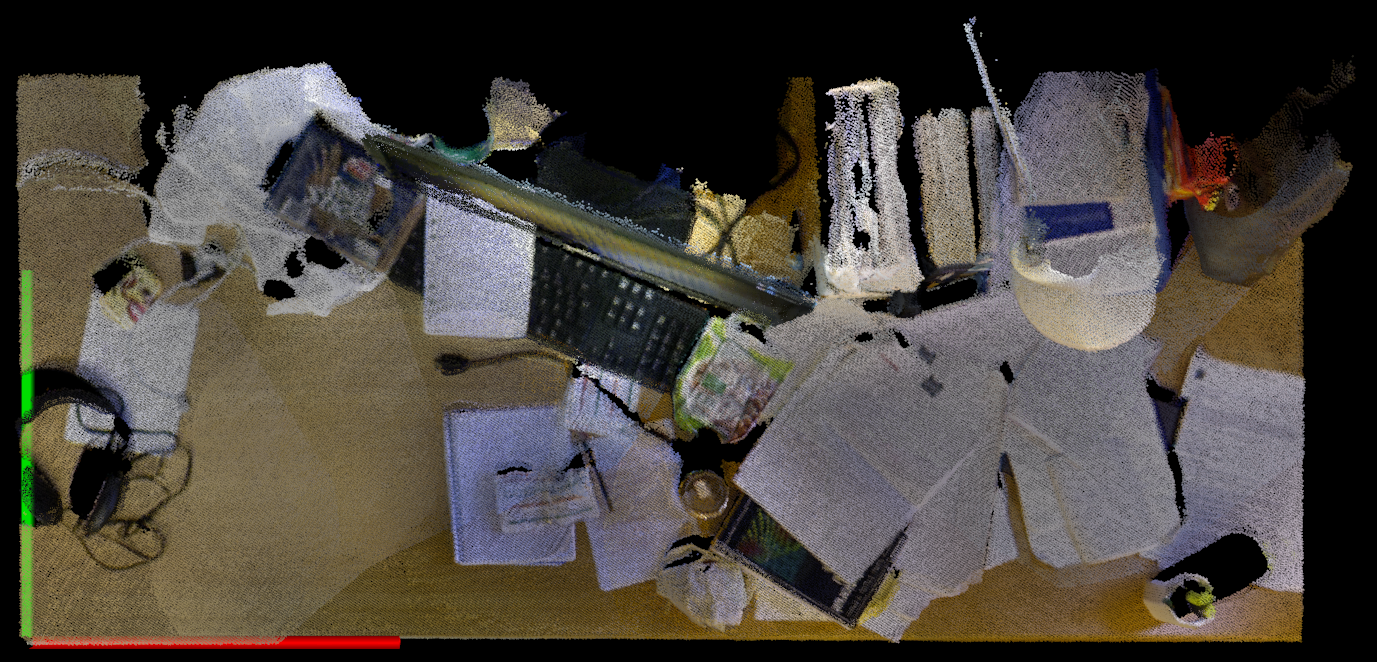
\includegraphics[height=2.5cm]{Puren_Mor_131110}
\caption{Each column shows a different person's office table at two different times. The tables in the first two columns are captured in the morning and evening of the same day, whereas the table in the last column is captured 12 days apart. We can see distinct differences between different person's table but there are also many commonalities that a system should exploit.}
\label{fig:Example Scenes}
\end{center}
\end{figure*}

\section{Related Work}
\label{sec:Related Work}
Learning a model for a type of scene is a difficult task if the raw data
acquired by the sensors is used in terms of metric measurements. Many
recent works have investigated how learning and modelling human
environments increase in efficacy if qualitative spatial features are
used instead of and/or alongside, metric ones. Spatial relations have been used
previously to provide contextual information to vision-related
work;~\cite{MyungJin:CVPR2010} used a hierarchy of spatial relations
alongside descriptive features to support multiple object detections
in a single image. Spatial relations and contextual information are
commonly used in activity recognition from video
streams~\cite{Krishna:ECAI2010, Behera2012}. Recent work has used
object co-occurrence to provide contexts in visual tasks such as
activity recognition~\cite{Li:2012}. Apart from using the mere
statistics of co-occurrence, a lot of information can be exploited
from \textit{how} the objects co-occur in the scene. Recent work in 3D
semantic labelling has used such geometric information along with
descriptive intrinsic appearance
features~\cite{Koppula:NIPS2011}. They achieve a high classification
accuracy for a large set of object-classes belonging to home and
office environments. Scene similarity measurement and classification
based on contextual information is conducted
by~\cite{Fisher:ACMT2011}. In~\cite{Aydemir:ICRA2011}, spatial
relations between smaller objects, furniture and locations is used for
pruning -- in object search problems in human
environments. In~\cite{Southey:2007,kasper:2011} the authors utilise
both geometric features on objects and spatial relations between
objects for scene understanding.

As described in the introduction our aim is to find and exploit the
spatial structures inherent in indoor environments. Three important
aspects are: complete scenes, same scenes observed over long times 
and to many similar but not identical scenes. Several datasets have 
been constructed for various researches. However, these existing 
datasets lack these three important aspects together.

The \textit{B3DO dataset}~\cite{Janoch:ICCV2011} contains many
single-snapshot instances of indoor human environments having a
variety in viewpoints, object-classes, scene-classes and
instances. This dataset is in the form of RGB and depth image pairs
with manual 2D annotations of object classes. It captures single
snapshots of unique scenes for which scene classification and object
classification is difficult for vision based perception systems (VPS).
The \textit{NYU Depth V1-2}~\cite{Silberman:ECCV2012} datasets contain
different instance examples of object-classes and scene-classes
captured with RGB+D images. Automated pixel clustering is conducted by
using features in the RGB and D images separately and annotation of
the clusters has been done manually, thereby assigning a semantic
label to every pixel. The dataset contains a wide range of singular
snapshots of indoor scenes from commercial and residential
buildings. This dataset is primarily aimed at evaluating VPS aiming at
automatic semantic segmentation and scene classification.

The \textit{3D IKEA database}~\cite{Swadzba:RAS2012} has been collected using a robot -- moving in different scene-class instances. The 
aim is to test scene-classification algorithms based on large, furniture level objects. 3D point clouds are formed by 
stitching a series of RGB+D images. There are very few small objects in the scenes and the annotations are provided at the 
scene-class level. The \textit{WRGBD dataset}~\cite{Lai:ICRA2011} is aimed to support object classification methods and contains many scene 
instances of isolated objects in point cloud format. Annotation is done by assigning every pixel a semantic label in each scene. Each point 
cloud is created from a series of RGB+D images.

The system constructed by~\cite{Russell:CVPR2009} can be used to automatically generate 3D datasets of scenes using rough human annotations 
on 2D images as input. The system infers 3D information from the scene using the semantics of the annotated properties of important planes 
in the image. The generated dataset thus includes a large set of singular scenes, indoor and outdoor from very particular viewpoints, with 
annotations to the image components provided manually.

The \textit{Kinect@Home project}~\cite{Goransson13a} has collected a large set of crowd sourced data. People having access to a kinect like sensor 
have captured and uploaded data from their own environments. The data is in the form of RGB-D video sequences. The data covers a large 
variety of different scene types and range from single objects to whole rooms. No annotation is available.
The dataset provided by~\cite{Sun:ECCV2010} contains a collection of 3D images of a few table-top objects in clear view and cluttered view. 
This dataset has been constructed to aid VPS for object classification and segmentation functioning on 3D data. Other datasets that have 
been developed have mainly been for training VPS for robust indoor object classification on 3D data~\cite{WillowGarage:2011,Kimmel:ACCV2010}.

Thusly, our dataset contributes with the following three important properties:
\begin{itemize}
	\item captures full 3D scene instances of a particular scene type (in our case office table-tops)
	\item contains instances of subsets of objects-of-interest co-occurring in the scenes -- manually annotated for ground truth
	\item provides long-term periodic observations of the same set of scenes at different times of the day, for several days.
\end{itemize}

Our dataset opens up the possibility to study the structures that govern how space is organised. We want to extract and later exploit these 
when building the models. While our dataset only captures table-tops we believe that many of our findings can be transferred to other types 
of scenes. As mentioned above, we expect most tables to have a monitor, a keyboard and a mouse and that these are arranged in a certain way. 
Many people will have the mouse to the right of the keyboard. This is an example of a spatial structure we want to learn. Some people have a 
laptop on their table and they bring this laptop home in the evening. This is an example of a dynamic property of a table that we want to 
learn. We believe that, when combined, this type of information will allow us to reason about activities as well.

Another aim is to be able to transfer knowledge from one part of an
environment to another and ultimately from one environment to the
next. For example, if the robot encounters a table that it has not seen
before, it should be able to make use of the models of other tables to
get a good prior for what to expect. In the same way that the reader
can form a mental picture of a typical office table arrangement.
This way, the robot would also be able to reason more efficiently
about tables that it has not yet seen but which, for example, might be
referenced by a human.

In conclusion, our dataset allows us to provide training data 
for spatial understanding models and spatial relations. It also helps 
to develop representations that caters for: knowledge transfer, 
the ability to learn from few samples and adapting existing models.

%%%%%%%%%%%%%%%%%%%%%%%%%%%%%%%%%%%%%%%%%%%%%%%%%%%%%%%%%%%%%%%%%%%%%%%%%%%%%%%%

\section{Dataset}
\label{sec:Dataset}
We focus on table-top scenes in our dataset because in an office 
environment the tables represent the work space of people. Each 
table-top is unique to that person but still similar to the others 
semantically and continuously changing. Table-tops are also well 
defined spatially and there are many instances of them within a 
single environment which means that capturing variation across 
instances is made more convenient.

With the aim of exploring possibilities to understand, learn and model these organisational structures amongst objects in human indoor 
environments, we present the dataset KTH-3D-TOTAL, which has been composed by periodically capturing observations of a fixed set of entire 
table-tops in an office environment. In what follows, we define a \textit{scene} as a single observation of a table-top instance at a single 
instance in time. The dataset captures the individual and group variations in object pose due to humans and their regular/irregular interaction with their environment. The 
required regularity in instances and time was the main motivation for the construction of this dataset, as currently available datasets 
either are of individual objects or single instances of tables or entire rooms. This regularity in sampling and extent over time is 
important when studying and modelling interrelations amidst the member objects in a long-term autonomous learning. 

\subsection{Dataset Design and Concept}
\label{ssec:Dataset Design and Concept}
We want to provide intelligence to a long-term operating, autonomous 
robot for indoor human environments. The KTH-3D-TOTAL dataset has 
been composed by capturing and manually annotating 3D point clouds 
of office type table-tops, for a fixed set of people, at fixed times of the 
day and for a span of weeks. Observing\footnote{Data collection protocol: At the 
designated collection times, people amidst their activities were asked to abruptly step 
aside from their tables and not allowed to alter the table-top or contribute to the 
occlusion of the table-top.} the table-tops of the same set of people at 
different times of the day gives insight about the daily interactions a 
human has with his table and over many days gives an understanding of the gradual 
variances of the configuration of these table-tops. If the data is observed for an entire week, 
including weekends, features in the table-top configurations, 
that can be used for estimation of the type of the day of the week, 
can be extracted (e.g.\ Weekdays, Fridays, Weekends). Table-top models can 
also be learnt for all the people put together -- which gives a gross functional
representation of an office table-top in general in office environments -- 
or for individual people which helps to build unique functional representations of 
office table-tops for individuals, for different activities and so on 
(Figure~\ref{fig:Example Scenes}). 
In summary: When the dataset is designed such that when it is partitioned in different ways with respect to time, people or object instances, it richly yields knowledge 
of table-tops in office environments supporting building representations of the same.

\subsection{Dataset Realization}
\label{ssec:Dataset Realization}
In KTH-3D-TOTAL, 3D point clouds representing 20 people's tables were captured regularly 3 times a day for 19 days. The data was collected by 
carefully scanning each table-top using an \textit{Asus Xtion Pro Live} RGB-D camera. The raw RGB-D data stream is aggregated into a single 
high resolution point cloud (.pcd format) using the \textit{SCENECT} software~\cite{Buerkler:Online2012}.

The scenes were recorded as periodically as possible and at three fixed times each day: \emph{Morning} (09:00 hrs), \emph{Afternoon} (13:00 
hrs) and \emph{Evening} (18:00 hrs). Scenes contain tables of 20 different people collected over 19 days including weekends. 
A \textit{Scene\_ID} is attached to each scene to indicate who the table belongs to and the date and time of the recording. These Scene\_IDs help in partitioning the dataset with respect to time of the day \{Morning, Afternoon, Evening\}, person \{Carl, Nils, \dots\}, or day \{2013-11-01, 2013-11-06, 2013-11-13, \dots\}.

A 3D annotation tool was developed for manually segmenting out objects-of-interest from the point clouds. On average, 12 different objects 
were labelled, including repeating instances of the same object class, per scene depending upon feasibility and occurrence. The objects 
belong to the following super set - \{Mouse, Keyboard, Monitor, Laptop, Cellphone, Keys, Headphones, Telephone, Pencil, Eraser, Notebook, 
Papers,  Book, Pen, Highlighter, Marker, Folder, Pen-Stand, Lamp, Mug, Flask, Glass, Jug, Bottle\}. The information about every scene and 
object is available in  XML and JSON formats. In these files, each scene has a nested list of object data containing \{Position, Orientation, Size, Date and 
Time of recording, Person ID, Point Indices of the points in the point cloud that have been labelled as belonging to the Object\}. This 
manual annotation provides the required ground truth data for long-term autonomous learning.

\subsection{Dataset Summary}
\label{ssec:Dataset Summary}
This section gives a bullet-summary of the dataset to serve as a quick reference.
\noindent KTH-3D-TOTAL has:
\begin{itemize}
	\item scenes collected from 20 unique tables, 3 times a day for 19 days and hence in total, approximately 1140 scenes.
	\item each scene manually annotated with 18 possible object classes and an average of 12 object instances, from these classes, annotated per scene, including multiple instances
	\item annotations stored in XML and JSON formats containing scene instance and it's object instances' specifications.
	\item occurrences of object instances as depicted in Figure~\ref{fig:HistOfObjects} and annotations as exemplified in Figure~\ref{fig:RawPCD},~\ref{fig:RawPCDAnnotated}
\end{itemize}

\begin{figure}[t]
\begin{center}
\subfloat[][]{\label{fig:HistOfObjects}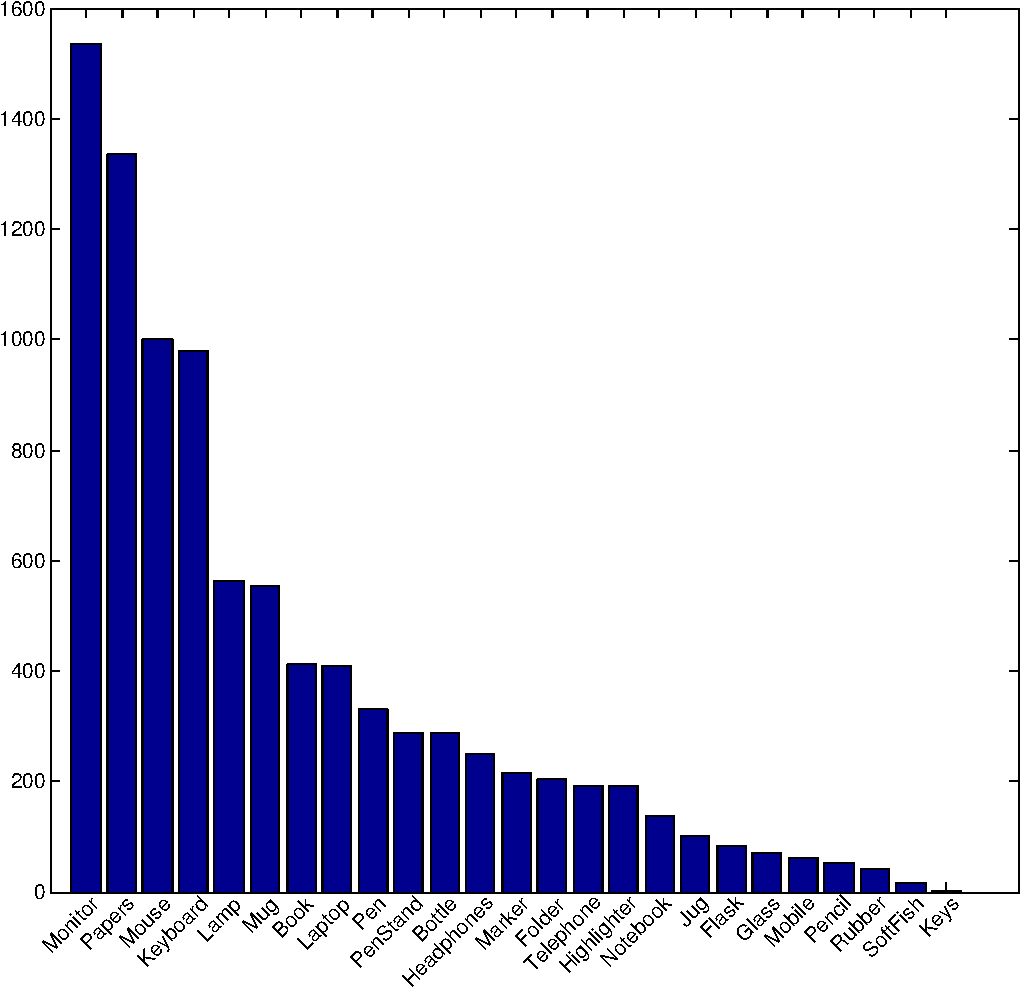
\includegraphics[width=0.8\linewidth]{HistOfObjects_crp.pdf}}\\
\subfloat[][]{\label{fig:RawPCD}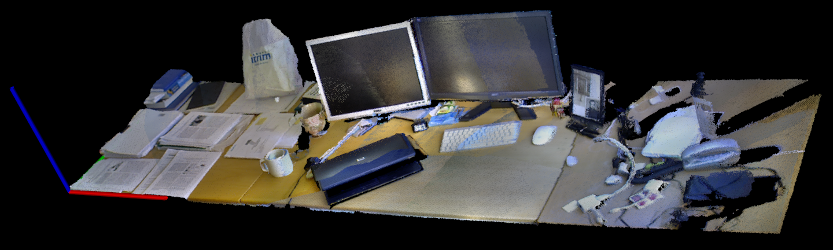
\includegraphics[width=0.7\linewidth]{pcd.png}}\\
\subfloat[][]{\label{fig:RawPCDAnnotated}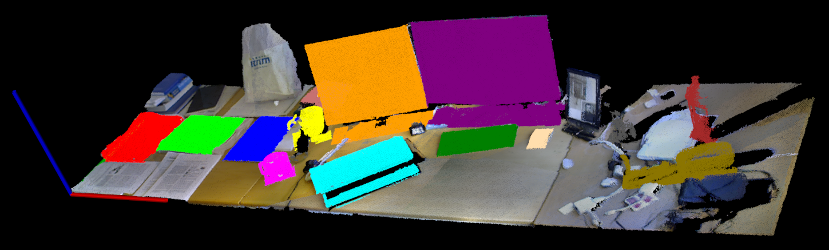
\includegraphics[width=0.7\linewidth]{pcd_annotated.png}}
\caption{(a) Objects annotated in 3D Long-Term Dataset, sorted in descending order of count of occurrences. X-axis$=$Object Name, Y-axis$=$Occurrence Count. (b) Screenshot of one table scene, along with it's annotations in (c).}
\end{center}
\end{figure}

%%%%%%%%%%%%%%%%%%%%%%%%%%%%%%%%%%%%%%%%%%%%%%%%%%%%%%%%%%%%%%%%%%%%%%%%%%%%%%%%

\section{Analysis}
\label{sec:Analysis}
In this section we perform an analysis of the data to highlight some
interesting aspects of it. In particular we will show that there are
structures in the data that can be exploited by a system for more
efficient representations and better reasoning with less data.  This
analysis then gives us insight into what we will later be able to
learn from this dataset and how to design such learning.

\begin{figure*}[bhtp]
\begin{center}
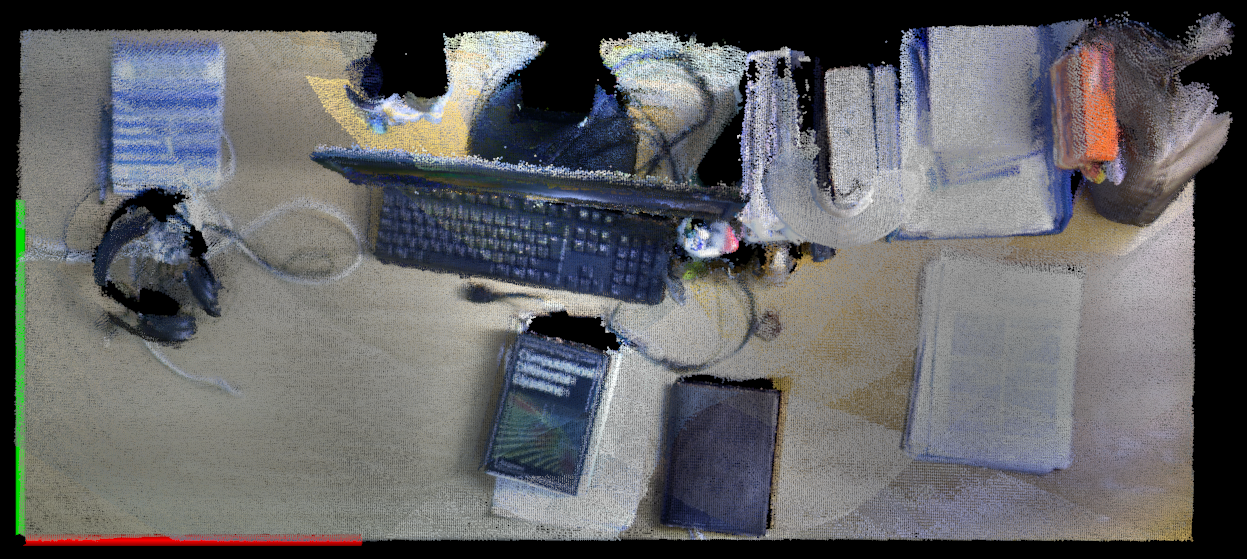
\includegraphics[height=2.5cm]{131024} \smallskip
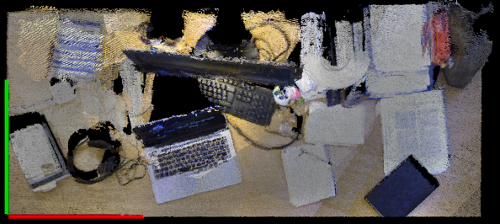
\includegraphics[height=2.5cm]{131028} \smallskip
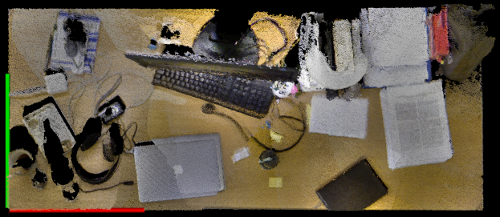
\includegraphics[height=2.5cm]{131108} \\
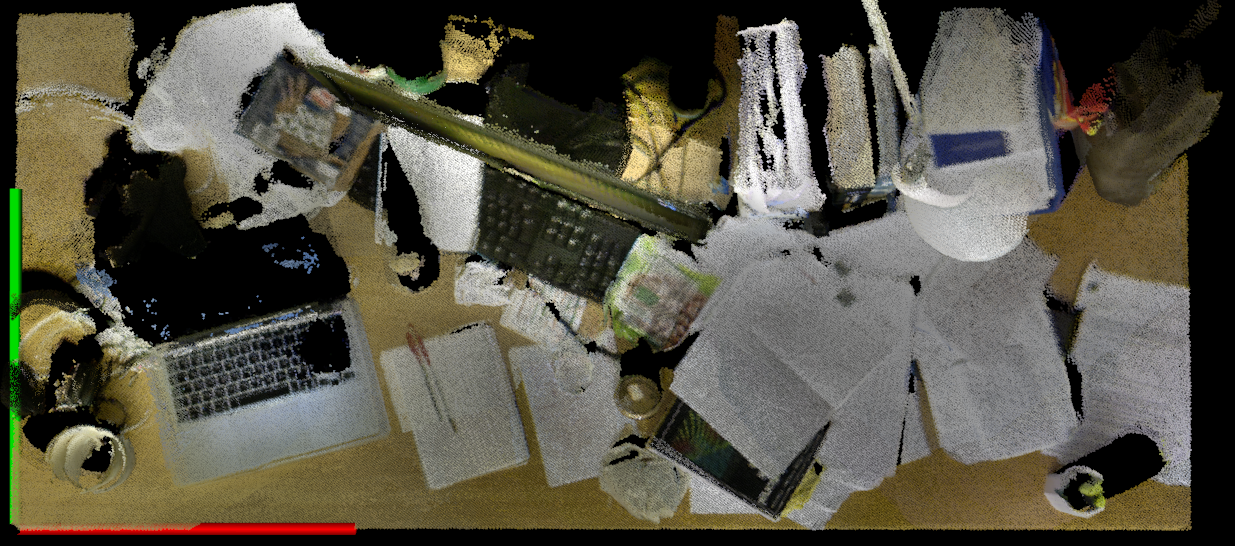
\includegraphics[height=2.5cm]{131113} \smallskip
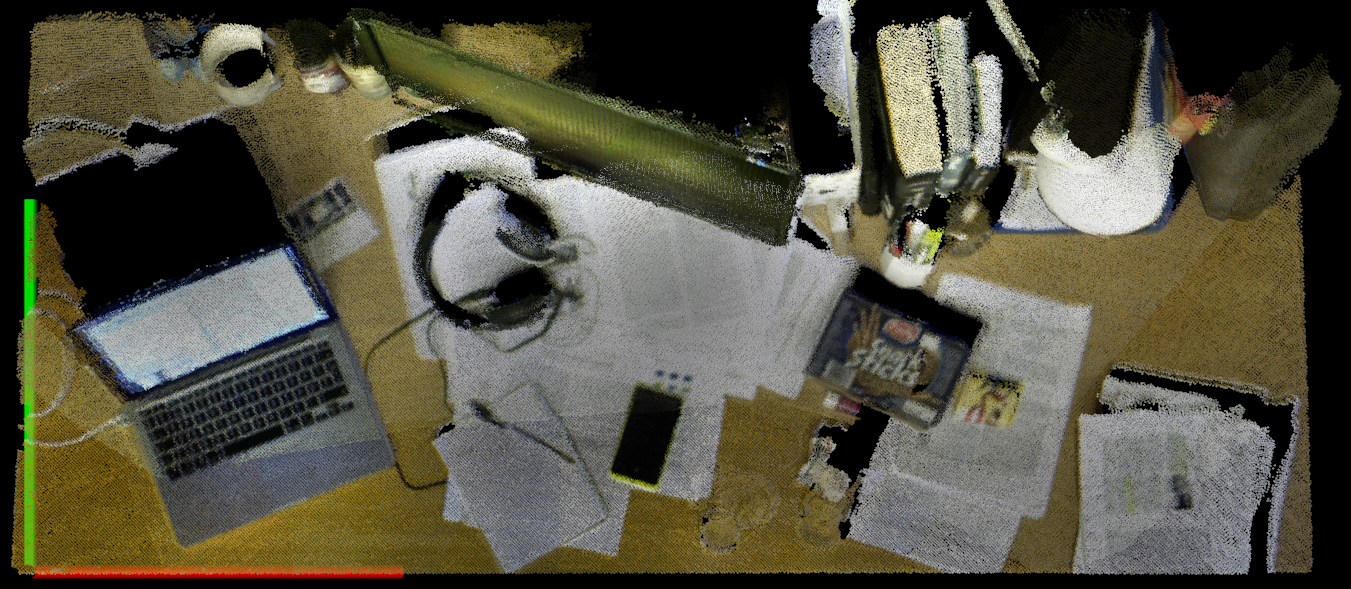
\includegraphics[height=2.5cm]{131114} \smallskip
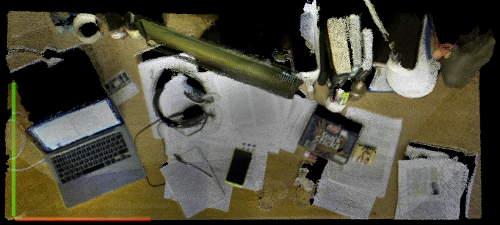
\includegraphics[height=2.5cm]{131116} 
\caption{This is the table of a single person, observed during the evening over many days: \{L to R -- Row 1: 24 Oct, 28 Oct, 08 Nov; Row 2: 13 Nov, 14 Nov, 16 Nov 2013\}. }
\label{fig:Variation_Over_Days}
\end{center}
\end{figure*}

Figure~\ref{fig:Example Scenes} shows three table-top scenes. Each column shows the same table at two different times. The leftmost two columns 
contain scenes from the same day, whereas the two scenes in the third column were sampled 12 days apart in time. Notice in Column 1: the slight changes in 
position of the keyboard, mouse, papers and pen; Column 2: the relatively big changes in position of laptop, mouse, papers, pen, keyboard, 
lamp. When objects in columns 1,2,3 are compared there is a certain generality in structure (keyboards are in front of monitors), but 
also a specificity for each person (occurrence of headphones, position of mouse w.r.t.\ keyboard, etc.). 

Studying the scenes could also allow a system to 
infer the activity of people. We can see that there are changes to the first table 
suggesting that someone was there during the day. Consider the table scenes in 
Figure~\ref{fig:Variation_Over_Days}, which captures the variations over the same person's
table over many days. Notice that between 28 Oct and 08 Nov the setup of the table does 
not change very much -- this reflects the ground truth that this person was working in 
another lab (room) and visited her table only to maybe, check emails. Now 
consider the variations between 08 Nov and 13 Nov -- this clearly indicates 
that the person was at her table and involved in working on the computer, 
reading and referring to papers and books, etc.\ There is a normal, day's 
worth of variation in between the images of 13 Nov and 14 Nov, however there 
is almost no variation between 14 Nov and 16 Nov -- which indicates that the 
person was absent over the weekend -- again a desirable property that ought 
to be captured by the long term autonomous systems.

Observing the tables can also infer a little about the working style of the 
people. In Figure~\ref{fig:Example Scenes}, the first table suggests that 
this person is tidy. The second table is missing the laptop in the second 
observation. This might suggest that 
the person has left the table, maybe for the day. The third table seems to 
be occupied by someone that is less sensitive to 
clutter. With only two observations of each tables these are just 
speculations but by looking at the data over 19 days stronger claims could be made.

One of our hypotheses is that a qualitative model will be needed to achieve 
efficient and powerful representations of 
space, at least if the amount of data is limited as it will be in realistic 
cases. Such qualitative models could allow some of the inherent 
structure in the environment be encoded in the representation itself. We 
have already seen in Figure~\ref{fig:Example Scenes} that monitors 
are typically at the rear end of the table, while a keyboard is usually in front of it and the 
leftmost table shows an example of a mouse ordinarily being to the right of a keyboard. 

Figure~\ref{fig:scatter-keyboard-mouse} shows a scatter plot 
over the position of keyboards and mice when found in the same scene. The 
table outline gives an example of a prototypical table to make it easier to 
interpret the data. 
In the top part of the figure, the green circles mark the position of the 
centroid of each 
keyboard that exist in a scene where there is at least one mouse. The red 
square shows the mean position of all these centroids. The black 
crosses show the position of all mice in scenes with at least one keyboard. 
In the bottom part of the figure the position of the mouse 
relative to the keyboard is shown for each observed pair in the data. As 
expected most mice are qualitatively to the right of the keyboard. There are 
some outliers. However,  
encoding the position of the mouse as being to the right of a keyboard would 
capture most of the information. The largest cluster of points in the lower 
part of Figure~\ref{fig:scatter-keyboard-mouse} contains about 95\% 
of all data points. Notice how this structure in the data is lost, at least 
visually, when looking at the position of the keyboard and mouse in the 
table frame (top figure) and how it pops out when looking at the relative 
positions (bottom figure). We want our representation to be able to 
capitalize on this structure. Clearly, in this case, the position of the 
keyboard contains almost all information that is needed to represent the 
position of the mouse as well. The figure also clearly shows how the 
distribution varies across person instances (the different colours in the bottom 
part). Note how each person has a lot less spread in the distribution than 
when considering them all at once. This is a good illustration of the 
difference between general models of space and models of specific instances 
of space; and the importance of the richness of the training data to provide for these two models.

\begin{figure}
\begin{center}
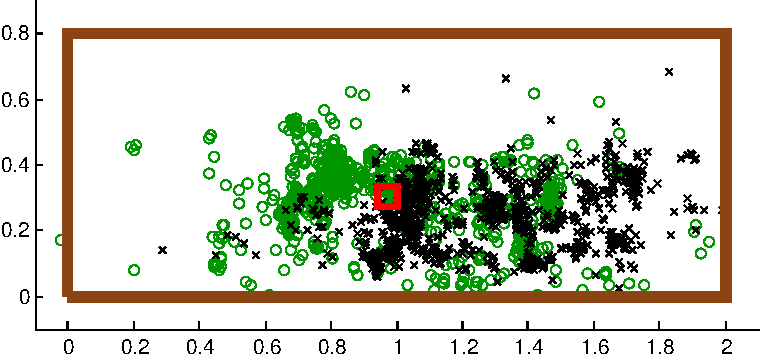
\includegraphics[width=0.8\linewidth]{keyboard_mouse_raw-crop}
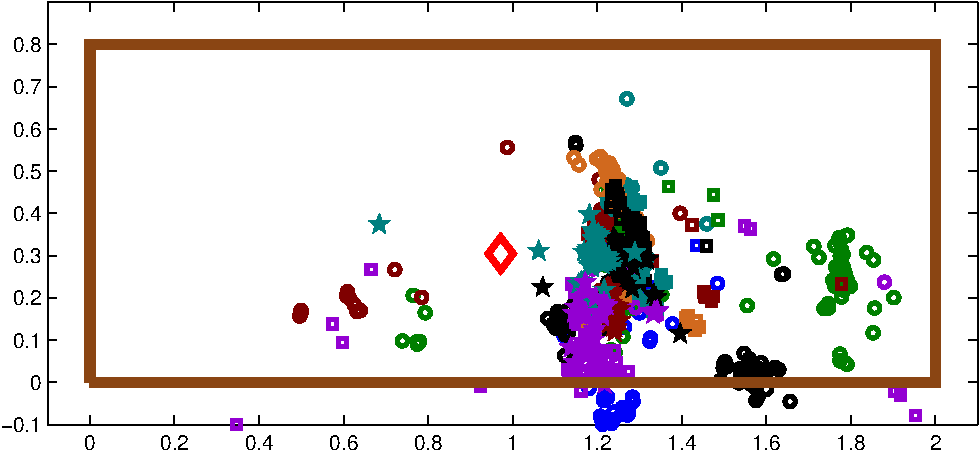
\includegraphics[width=0.8\linewidth]{clusters/plots-for-paper/keyboard_mouse_clusters-crop}
\end{center}
\caption{This figures shows how a relative position representation (bottom) 
is able to expose a structure that is not visible in absolute coordinated 
(top). 
Top: The green circles shows the positions keyboards(red square shows mean 
of keyboards). The black crosses show the position of all mice in these 
scenes. Bottom: Mean position of keyboards (red square) and relative 
position of mouse relative to it. Each color shows a different person. The 
brown rectangle gives a rough idea about where the borders of a typical 
table would be.} 
\label{fig:scatter-keyboard-mouse}
\end{figure}

To further investigate the correlation between different object classes, and 
thus look for other inherent structures in the data, we look at 
the relative position of all objects of class $C_j$ w.r.t.\ to objects of 
class $C_i$ present in the same scene and turn to information theory for the 
analysis. We calculate the entropy over the histogram of the distributions 
of relative positions (i.e.\ histogram over bottom figure in 
Figure~\ref{fig:scatter-keyboard-mouse}, for instance). Entropy measures the 
predictability of the information. A low entropy means that there are 
informative features available to make prediction, i.e. there is an 
underlying structure. A large entropy on the other hand means that it is 
very hard to make predictions and the resulting distribution would be close 
to uniform.
We calculate the entropy as 
\begin{equation}
E=-\sum (\frac{n_i}{N})ln(\frac{n_i}{N})
\end{equation}
where $n_i$ is the number of samples that fall in cell $i$ in a grid 
discretization of the table and N is the total number of samples. Each 
sample corresponds to one object pair in one scene. The true entropy will 
only be estimated well when $N$ is large. We therefore limit this 
investigation to pairs of objects that occur more than a certain number of 
times in the data. Figure~\ref{fig:entropy} shows these entropies 
for 10 of the objects in the dataset. From this figure we can, for example, 
see the low entropy in the relation between keyboard and mouse (elements 1,3 
and 3,1 in the matrix). The relative positions of monitors and keyboards 
also have a fairly low entropy. We also see that the 
position of papers is largely uncorrelated with many other objects (uniform 
distribution gives high entropy). The values from such an entropy matrix 
could give suggestions toward hypothesizing a possible hierarchy in data 
organisation for the robots. Those objects that have a lot of positional 
variance could be described as target objects with respect to landmark 
objects that do not vary as much. This organising tree structure could also 
potentially be autonomously learnt -- leading to more than one landmark object in a scene. A keyboard-mouse-monitor-laptop could be organised in a parallel sub-tree alongside a mug-glass-jug-flask sub-tree. We make these suggestions purely based on conjecture, which we aim to verify in our following research work.

In Figure~\ref{fig:scatter-rest} we look closer at some of these relations. 
Figure~\ref{fig:scatter-monitor-keyboard} shows the position of 
the keyboard w.r.t.\ to the monitors. Our intuition that keyboards are 
placed mostly in front of monitors is supported by data. 
Figure~\ref{fig:scatter-keyboard-mug} shows the position of the mug w.r.t\ 
the keyboard. We see that the mug is rarely very close to the center of the 
keyboard but rather positioned around the keyboard. Taking function into 
account the data might suggest that the mug 
is in fact often placed at arms length from the person working on the table 
to keep it at safe distance from the keyboard but still within 
reach. We see a bias towards the right side, probably a result of most 
people being right-handed. In Figure~\ref{fig:scatter-keyboard-papers} we see 
that the distribution for the relative position of papers w.r.t.\ to the 
keyboard is almost uniform, suggesting that they are largely uncorrelated. 
Upon keener observations we can see that there are some clusters of similar 
markers which indicate that papers are not as dynamic as the mouse or mug, 
and hold their place usually for a couple of days on average. 
The fact that there are often many papers in a scene adds to the uniformity.

%\begin{figure}
%\begin{center}
%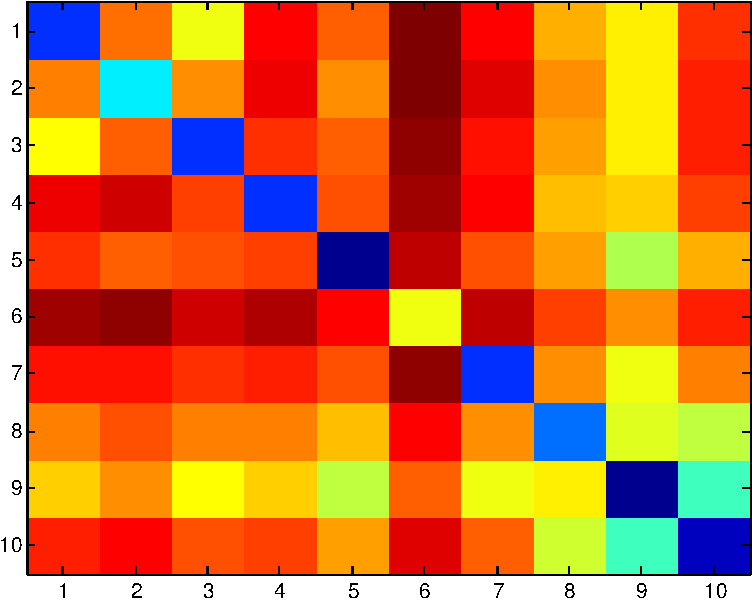
\includegraphics[width=\linewidth]{entropy_matrix-crop} \quad
%\begin{tabular}{|l||c|c|c|c|c|c|c|c|c|c|c|c|c|}
%\hline
%& key & mon & mou & mug & lap & pap & boo & bot & jug & not \\ \hline \hline
%key & 0.76 & 3.54 & 2.79 & 4.01 & 3.56 & 4.57 & 4.00 & 3.25 & 2.95 & 3.78\\ \hline
%mon & 3.41 & 1.65 & 3.35 & 4.06 & 3.39 & 4.63 & 4.19 & 3.37 & 2.95 & 3.86\\ \hline
%mou & 2.89 & 3.59 & 0.73 & 3.81 & 3.59 & 4.56 & 3.96 & 3.27 & 2.93 & 3.84 \\ \hline
%mug & 4.08 & 4.21 & 3.71 & 0.74 & 3.67 & 4.47 & 3.99 & 3.17 & 3.08 & 3.73 \\ \hline
%lap & 3.79 & 3.60 & 3.67 & 3.70 & 0.05 & 4.34 & 3.67 & 3.30 & 2.47 & 3.23 \\ \hline
%pap & 4.45 & 4.50 & 4.22 & 4.41 & 4.01 & 2.76 & 4.30 & 3.72 & 3.36 & 3.84 \\ \hline
%boo & 3.96 & 3.93 & 3.81 & 3.86 & 3.67 & 4.49 & 0.77 & 3.35 & 2.81 & 3.42 \\ \hline
%bot & 3.47 & 3.64 & 3.44 & 3.42 & 3.17 & 4.03 & 3.33 & 1.03 & 2.74 & 2.58 \\ \hline
%jug & 3.05 & 3.34 & 2.85 & 3.11 & 2.54 & 3.56 & 2.81 & 2.95 & 0.00 & 1.97 \\ \hline
%not & 3.90 & 3.99 & 3.68 & 3.70 & 3.29 & 4.16 & 3.59 & 2.62 & 1.97 & 0.28 \\ \hline
%\end{tabular}
%\end{center}
%\caption{The figure illustrates the entropy in the distribution of relative positions of one object (column) w.r.t. to another object (row). Dark red indicates high entropy (more uniform distr.) and dark blue low entropy (peakier distr.). We show this for the most frequently occurring object pairs in the dataset (i.e. most statistics); 1:keyboard, 2:monitor, 3:mouse, 4:mug, 5:laptop, 6:papers, 7:book, 8:bottle, 9:jug, 10:notebook. }
%\label{fig:entropy}
%\end{figure}

%\begin{figure*}
%\begin{center}
%\begin{tabular}{|l||c|c|c|c|c|c|c|c|c|c|c|c|c|}
%\hline
%& $C_{1}$ & $C_{2}$ & $C_{3}$ & $C_{4}$ & $C_{5}$ & $C_{6}$ & $C_{7}$ & $C_{8}$ & $C_{9}$ & $C_{10}$ \\ \hline \hline
%$C_1$: keyboard & 0.76 & 3.54 & 2.79 & 4.01 & 3.56 & 4.57 & 4.00 & 3.25 & 2.95 & 3.78\\ \hline
%$C_2$: monitor & 3.41 & 1.65 & 3.35 & 4.06 & 3.39 & 4.63 & 4.19 & 3.37 & 2.95 & 3.86\\ \hline
%$C_3$: mouse & 2.89 & 3.59 & 0.73 & 3.81 & 3.59 & 4.56 & 3.96 & 3.27 & 2.93 & 3.84 \\ \hline
%$C_4$: mug & 4.08 & 4.21 & 3.71 & 0.74 & 3.67 & 4.47 & 3.99 & 3.17 & 3.08 & 3.73 \\ \hline
%$C_5$: laptop & 3.79 & 3.60 & 3.67 & 3.70 & 0.05 & 4.34 & 3.67 & 3.30 & 2.47 & 3.23 \\ \hline
%$C_6$: papers & 4.45 & 4.50 & 4.22 & 4.41 & 4.01 & 2.76 & 4.30 & 3.72 & 3.36 & 3.84 \\ \hline
%$C_7$: book & 3.96 & 3.93 & 3.81 & 3.86 & 3.67 & 4.49 & 0.77 & 3.35 & 2.81 & 3.42 \\ \hline
%$C_{8}$: bottle & 3.47 & 3.64 & 3.44 & 3.42 & 3.17 & 4.03 & 3.33 & 1.03 & 2.74 & 2.58 \\ \hline
%$C_{9}$: jug & 3.05 & 3.34 & 2.85 & 3.11 & 2.54 & 3.56 & 2.81 & 2.95 & 0.00 & 1.97 \\ \hline
%$C_{10}$: notebook & 3.90 & 3.99 & 3.68 & 3.70 & 3.29 & 4.16 & 3.59 & 2.62 & 1.97 & 0.28 \\ \hline
%\end{tabular}
%\label{fig:entropy}
%\caption{The table shows the entropy in the spread in positions that results when looking at the position of one object (columns) with respect to that of another one (rows). As we can see papers have high entropy in combination with all other objects which indicates that the distribution of relative positions is close to uniform. Other combinations such as Keyboard and Mouse have much lower entropy, that is, more peaky distribution showing a stronger correlation.}
%\end{center}
%\end{figure*}

\begin{figure*}
\begin{center}
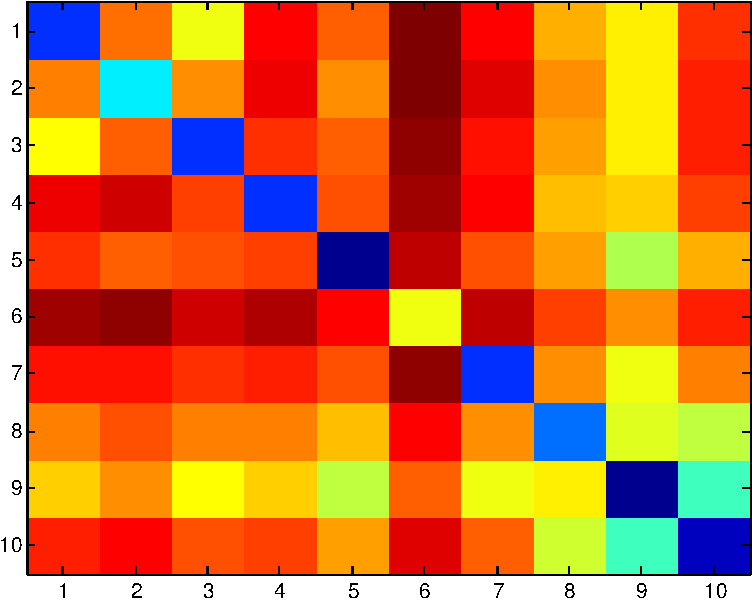
\includegraphics[width=0.5\linewidth]{entropy_matrix-crop} \bigbreak
\begin{tabular}{|l||c|c|c|c|c|c|c|c|c|c|c|c|c|}
\hline
& key & mon & mou & mug & lap & pap & boo & bot & jug & not \\ \hline \hline
key & 0.76 & 3.54 & 2.79 & 4.01 & 3.56 & 4.57 & 4.00 & 3.25 & 2.95 & 3.78\\ \hline
mon & 3.41 & 1.65 & 3.35 & 4.06 & 3.39 & 4.63 & 4.19 & 3.37 & 2.95 & 3.86\\ \hline
mou & 2.89 & 3.59 & 0.73 & 3.81 & 3.59 & 4.56 & 3.96 & 3.27 & 2.93 & 3.84 \\ \hline
mug & 4.08 & 4.21 & 3.71 & 0.74 & 3.67 & 4.47 & 3.99 & 3.17 & 3.08 & 3.73 \\ \hline
lap & 3.79 & 3.60 & 3.67 & 3.70 & 0.05 & 4.34 & 3.67 & 3.30 & 2.47 & 3.23 \\ \hline
pap & 4.45 & 4.50 & 4.22 & 4.41 & 4.01 & 2.76 & 4.30 & 3.72 & 3.36 & 3.84 \\ \hline
boo & 3.96 & 3.93 & 3.81 & 3.86 & 3.67 & 4.49 & 0.77 & 3.35 & 2.81 & 3.42 \\ \hline
bot & 3.47 & 3.64 & 3.44 & 3.42 & 3.17 & 4.03 & 3.33 & 1.03 & 2.74 & 2.58 \\ \hline
jug & 3.05 & 3.34 & 2.85 & 3.11 & 2.54 & 3.56 & 2.81 & 2.95 & 0.00 & 1.97 \\ \hline
not & 3.90 & 3.99 & 3.68 & 3.70 & 3.29 & 4.16 & 3.59 & 2.62 & 1.97 & 0.28 \\ \hline
\end{tabular}\bigbreak
\caption{The figure illustrates the entropy value in the distribution of relative positions of one object (column) w.r.t. to another object (row). Dark red indicates high entropy (more uniform distribution) and dark blue low entropy (more peaky distribution). We show this for the most frequently occurring object pairs in the dataset (i.e. most statistics). The table shows the actual entropy values corresponding to the above illustration.}
\label{fig:entropy}
\end{center}
\end{figure*}

%\begin{itemize}	
%\item keyboard
%\item monitor
%\item mouse
%\item mug
%\item laptop
%\item papers
%\item book
%\item bottle
%\item jug
%\item notebook
%\item mobile
%\item glass
%\item flask
%\end{itemize}

\begin{figure}[t]
\begin{center}
\subfloat[][]{\label{fig:scatter-monitor-keyboard}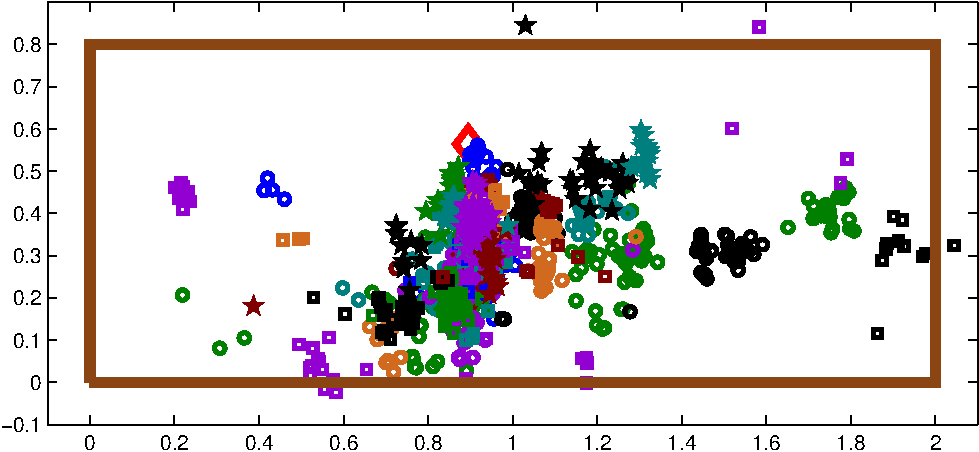
\includegraphics[width=0.8\linewidth]{clusters/plots-for-paper/monitor_keyboard_clusters-crop}}\quad
\subfloat[][]{\label{fig:scatter-keyboard-mug}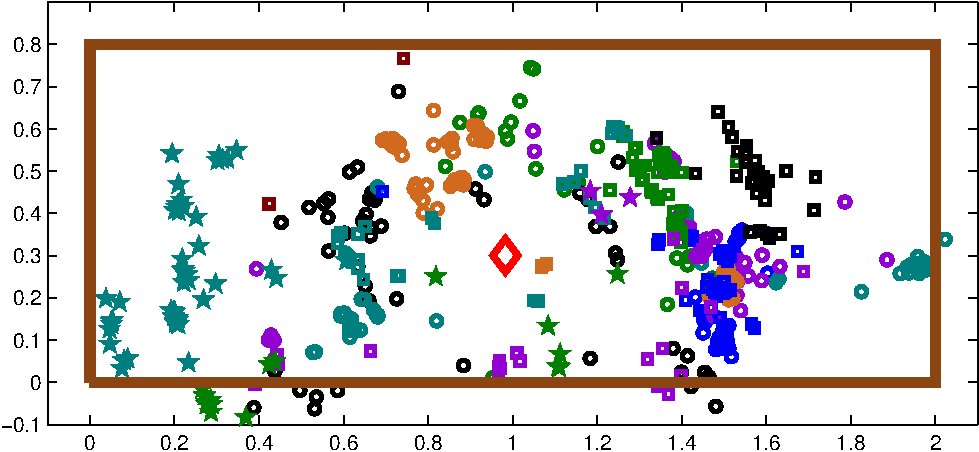
\includegraphics[width=0.8\linewidth]{clusters/plots-for-paper/keyboard_mug_clusters-crop}}\\
\subfloat[][]{\label{fig:scatter-keyboard-papers}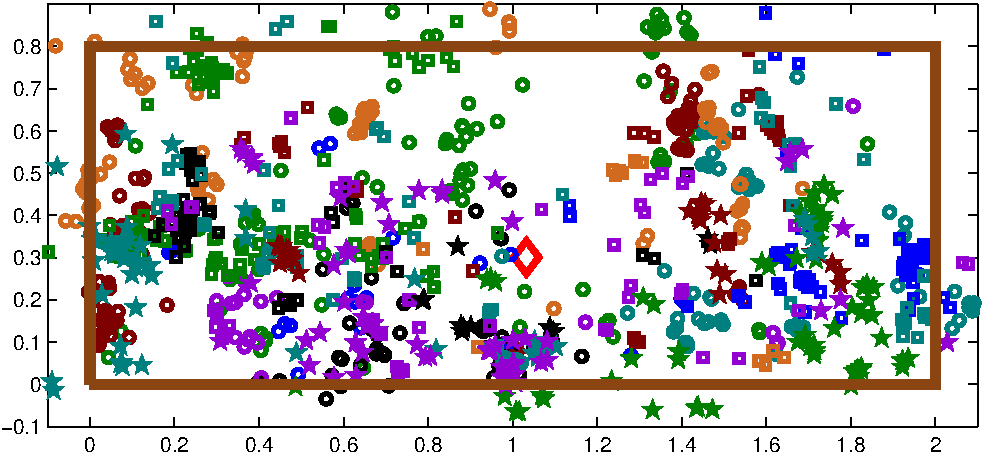
\includegraphics[width=0.8\linewidth]{clusters/plots-for-paper/keyboard_papers_clusters-crop}}
\end{center}
\caption{The figures show the relative position of a) keyboard w.r.t. monitor, b) mug w.r.t. keyboard and c) papers w.r.t. keyboard. Qualitatively keyboards are mostly infront of monitors, mugs are around the keyboard and the position of papers is mostly independent on the position of the keyboard. The different colors/markers show data from different people in the data.} 
\label{fig:scatter-rest}
\end{figure}

To summarize the analysis, we have shown that the data has many structural 
properties that a method for representing and reasoning about 
space should exploit. If the aim is to represent typical configuration of 
objects, this preliminary analysis suggests that a significant 
part of such knowledge can be encoded well with qualitative spatial 
relations, such as the mouse is to the \textit{right of} the keyboard, while 
keeping in mind that this represents the typical case and not the only 
possible situation. We can also see that a system that observes these tables for 
an extended period of time will be able to learn quite a lot about the 
habits of the owners of the tables and even the current activity in 
many cases. It is important to differentiate between typical knowledge, 
i.e., knowledge about what the world typically is like and specific 
instance knowledge, i.e., knowledge about a particular scene at a specific 
time. It is to capture the first kind of knowledge that we 
believe  qualitative spatial representations will be most beneficial. 

%%%%%%%%%%%%%%%%%%%%%%%%%%%%%%%%%%%%%%%%%%%%%%%%%%%%%%%%%%%%%%%%%%%%%%%%%%%%%%%%
\section{Conclusions}
\label{sec:Conclusions}

We have shown that there is structure in the way that objects are
arranged in scenes.  We can expect that robots operating over long periods 
of time, repeatedly observing the same scenes and types of scenes, 
will be able to learn models of this structure -- preserving the temporal 
and instance variations in the scenes. 
The large, manually annotated, benchmark 3D dataset we present, is one-of-a-kind -- 
providing the means to train long-term autonomous learning systems for spatial understanding.

Our immediate research plans for this data are to learn and model the spatial relations amidst objects contained in the scenes. Such models and spatial relations can subsequently be tested, verified and also used by the autonomous robots in our collaborative research project (STRANDS) while they operate over months at various sites.  These will
allow for activity recognition, anomaly detection, and context recognition which are the crux of such long-term autonomous service robots.

%%%%%%%%%%%%%%%%%%%%%%%%%%%%%%%%%%%%%%%%%%%%%%%%%%%%%%%%%%%%%%%%%%%%%%%%%%%%%%%%
\section{Acknowledgements}
\label{sec:Acknowledgements}

The research leading to these results has received funding from the European
Union Seventh Framework Programme (FP7/2007-2013) under grant agreement No 600623, STRANDS,
the Swedish Research Council and the Swedish Foundation for Strategic Research through its Centre for Autonomous Systems.
We thank CVAP/CAS, KTH Royal Institute of technology, Stockholm, Sweden for participating in the dataset and Accel Partners, Bangalore, India for providing vital logistical help.

\bibliographystyle{ieeetr}
\bibliography{references}

\end{document}